% Options for packages loaded elsewhere
\PassOptionsToPackage{unicode}{hyperref}
\PassOptionsToPackage{hyphens}{url}
\PassOptionsToPackage{dvipsnames,svgnames,x11names}{xcolor}
%
\documentclass[
  ignorenonframetext,
]{beamer}
\usepackage{pgfpages}
\setbeamertemplate{caption}[numbered]
\setbeamertemplate{caption label separator}{: }
\setbeamercolor{caption name}{fg=normal text.fg}
\beamertemplatenavigationsymbolsempty
% Prevent slide breaks in the middle of a paragraph
\widowpenalties 1 10000
\raggedbottom

\usepackage{amsmath,amssymb}
\usepackage{iftex}
\ifPDFTeX
  \usepackage[T1]{fontenc}
  \usepackage[utf8]{inputenc}
  \usepackage{textcomp} % provide euro and other symbols
\else % if luatex or xetex
  \usepackage{unicode-math}
  \defaultfontfeatures{Scale=MatchLowercase}
  \defaultfontfeatures[\rmfamily]{Ligatures=TeX,Scale=1}
\fi
\usepackage{lmodern}
\usetheme[]{AnnArbor}
\usecolortheme{dolphin}
\usefonttheme{structurebold}
\ifPDFTeX\else  
    % xetex/luatex font selection
\fi
% Use upquote if available, for straight quotes in verbatim environments
\IfFileExists{upquote.sty}{\usepackage{upquote}}{}
\IfFileExists{microtype.sty}{% use microtype if available
  \usepackage[]{microtype}
  \UseMicrotypeSet[protrusion]{basicmath} % disable protrusion for tt fonts
}{}
\makeatletter
\@ifundefined{KOMAClassName}{% if non-KOMA class
  \IfFileExists{parskip.sty}{%
    \usepackage{parskip}
  }{% else
    \setlength{\parindent}{0pt}
    \setlength{\parskip}{6pt plus 2pt minus 1pt}}
}{% if KOMA class
  \KOMAoptions{parskip=half}}
\makeatother
\usepackage{xcolor}
\newif\ifbibliography
\setlength{\emergencystretch}{3em} % prevent overfull lines
\setcounter{secnumdepth}{-\maxdimen} % remove section numbering


\providecommand{\tightlist}{%
  \setlength{\itemsep}{0pt}\setlength{\parskip}{0pt}}\usepackage{longtable,booktabs,array}
\usepackage{calc} % for calculating minipage widths
\usepackage{caption}
% Make caption package work with longtable
\makeatletter
\def\fnum@table{\tablename~\thetable}
\makeatother
\usepackage{graphicx}
\makeatletter
\def\maxwidth{\ifdim\Gin@nat@width>\linewidth\linewidth\else\Gin@nat@width\fi}
\def\maxheight{\ifdim\Gin@nat@height>\textheight\textheight\else\Gin@nat@height\fi}
\makeatother
% Scale images if necessary, so that they will not overflow the page
% margins by default, and it is still possible to overwrite the defaults
% using explicit options in \includegraphics[width, height, ...]{}
\setkeys{Gin}{width=\maxwidth,height=\maxheight,keepaspectratio}
% Set default figure placement to htbp
\makeatletter
\def\fps@figure{htbp}
\makeatother
% definitions for citeproc citations
\NewDocumentCommand\citeproctext{}{}
\NewDocumentCommand\citeproc{mm}{%
  \begingroup\def\citeproctext{#2}\cite{#1}\endgroup}
\makeatletter
 % allow citations to break across lines
 \let\@cite@ofmt\@firstofone
 % avoid brackets around text for \cite:
 \def\@biblabel#1{}
 \def\@cite#1#2{{#1\if@tempswa , #2\fi}}
\makeatother
\newlength{\cslhangindent}
\setlength{\cslhangindent}{1.5em}
\newlength{\csllabelwidth}
\setlength{\csllabelwidth}{3em}
\newenvironment{CSLReferences}[2] % #1 hanging-indent, #2 entry-spacing
 {\begin{list}{}{%
  \setlength{\itemindent}{0pt}
  \setlength{\leftmargin}{0pt}
  \setlength{\parsep}{0pt}
  % turn on hanging indent if param 1 is 1
  \ifodd #1
   \setlength{\leftmargin}{\cslhangindent}
   \setlength{\itemindent}{-1\cslhangindent}
  \fi
  % set entry spacing
  \setlength{\itemsep}{#2\baselineskip}}}
 {\end{list}}
\usepackage{calc}
\newcommand{\CSLBlock}[1]{\hfill\break\parbox[t]{\linewidth}{\strut\ignorespaces#1\strut}}
\newcommand{\CSLLeftMargin}[1]{\parbox[t]{\csllabelwidth}{\strut#1\strut}}
\newcommand{\CSLRightInline}[1]{\parbox[t]{\linewidth - \csllabelwidth}{\strut#1\strut}}
\newcommand{\CSLIndent}[1]{\hspace{\cslhangindent}#1}

\usepackage{booktabs}
\usepackage{longtable}
\usepackage{array}
\usepackage{multirow}
\usepackage{wrapfig}
\usepackage{float}
\usepackage{colortbl}
\usepackage{pdflscape}
\usepackage{tabu}
\usepackage{threeparttable}
\usepackage{threeparttablex}
\usepackage[normalem]{ulem}
\usepackage{makecell}
\usepackage{xcolor}

% logo
\titlegraphic{
\includegraphics[width=4cm]{000_logos/logo-blue-vertical}}
\logo{\ifnum\thepage>1
\includegraphics[width=0.5cm]{000_logos/logo-blue-vertical}\fi}

% UMNG: Manual de image institucional

% Colors

% Umng
\definecolor{yellow}{HTML}{fdc600}
\definecolor{red}{HTML}{ee2a24}

% Estudios a Distancia
\definecolor{blue1}{HTML}{12245b}
\definecolor{blue2}{HTML}{767ca6}
\definecolor{blue3}{HTML}{cad2ec}

% Modify items
\setbeamercolor{palette primary}{bg=blue3}
\setbeamercolor{palette tertiary}{bg=blue1}
\setbeamercolor{frametitle}{bg=yellow}

% Hyperlinks
\hypersetup{
  linkcolor=red,
  citecolor=red
}

\makeatletter
\@ifpackageloaded{caption}{}{\usepackage{caption}}
\AtBeginDocument{%
\ifdefined\contentsname
  \renewcommand*\contentsname{Table of contents}
\else
  \newcommand\contentsname{Table of contents}
\fi
\ifdefined\listfigurename
  \renewcommand*\listfigurename{List of Figures}
\else
  \newcommand\listfigurename{List of Figures}
\fi
\ifdefined\listtablename
  \renewcommand*\listtablename{List of Tables}
\else
  \newcommand\listtablename{List of Tables}
\fi
\ifdefined\figurename
  \renewcommand*\figurename{Figure}
\else
  \newcommand\figurename{Figure}
\fi
\ifdefined\tablename
  \renewcommand*\tablename{Table}
\else
  \newcommand\tablename{Table}
\fi
}
\@ifpackageloaded{float}{}{\usepackage{float}}
\floatstyle{ruled}
\@ifundefined{c@chapter}{\newfloat{codelisting}{h}{lop}}{\newfloat{codelisting}{h}{lop}[chapter]}
\floatname{codelisting}{Listing}
\newcommand*\listoflistings{\listof{codelisting}{List of Listings}}
\makeatother
\makeatletter
\makeatother
\makeatletter
\@ifpackageloaded{caption}{}{\usepackage{caption}}
\@ifpackageloaded{subcaption}{}{\usepackage{subcaption}}
\makeatother

\ifLuaTeX
\usepackage[bidi=basic]{babel}
\else
\usepackage[bidi=default]{babel}
\fi
\babelprovide[main,import]{english}
% get rid of language-specific shorthands (see #6817):
\let\LanguageShortHands\languageshorthands
\def\languageshorthands#1{}
\ifLuaTeX
  \usepackage{selnolig}  % disable illegal ligatures
\fi
\usepackage{bookmark}

\IfFileExists{xurl.sty}{\usepackage{xurl}}{} % add URL line breaks if available
\urlstyle{same} % disable monospaced font for URLs
\hypersetup{
  pdftitle={Money, prices and the exchange rate},
  pdfauthor={Luis Francisco Gómez López},
  pdflang={en},
  colorlinks=true,
  linkcolor={Maroon},
  filecolor={Maroon},
  citecolor={Blue},
  urlcolor={Blue},
  pdfcreator={LaTeX via pandoc}}


\title{Money, prices and the exchange rate}
\author{Luis Francisco Gómez López}
\date{2024-07-17}
\institute{FAEDIS}

\begin{document}
\frame{\titlepage}

\renewcommand*\contentsname{Table of contents}
\begin{frame}[allowframebreaks]
  \frametitle{Table of contents}
  \tableofcontents[hideallsubsections]
\end{frame}

\section{Please Read Me}\label{please-read-me}

\begin{frame}{}
\phantomsection\label{section}
\begin{itemize}
\item
  Check the message \textbf{Welcome greeting} published in the News
  Bulletin Board.
\item
  Dear student please edit your profile uploading a photo where your
  face is clearly visible.
\item
  The purpose of the virtual meetings is to answer questions and not to
  make a summary of the study material.
\item
  This presentation is based on
  (\citeproc{ref-cardenas_introduccion_2020}{Cardenas 2020, chap. 7})
\end{itemize}
\end{frame}

\section{Purpose}\label{purpose}

\begin{frame}{}
\phantomsection\label{section-1}
Analyze the money market and introduce the concepts of inflation,
nominal exchange rate and interest rate
\end{frame}

\section{Money and Central Banks}\label{money-and-central-banks}

\begin{frame}{}
\phantomsection\label{section-2}
\begin{itemize}
\item
  Money is an \textbf{asset} that fulfills in general 3 functions

  \begin{itemize}
  \tightlist
  \item
    Medium of exchange
  \item
    Unit of account
  \item
    Store of value
  \end{itemize}
\item
  A central bank\footnote<.->{For a list of central banks around the
    world see
    \href{https://www.bis.org/cbanks.htm}{\textbf{https://www.bis.org/cbanks.htm}}}
  is the institution that issues and administrates legal currency and
  exercises the function of banker of banks
  (\citeproc{ref-banco_de_la_republica_central_2021}{República 2021})
\item
  In the case of Colombia, some of the functions of the central bank
  are:

  \begin{itemize}
  \tightlist
  \item
    Keep inflation low and stable and achieve the highest sustainable
    level of output and employment
  \item
    Manage international reserves
  \item
    Act as the bank of bankers
  \item
    Issue currency
  \item
    Act as a government banker, fiscal agent and trustee
  \end{itemize}
\end{itemize}
\end{frame}

\begin{frame}{}
\phantomsection\label{section-3}
\begin{table}

\caption{\label{tbl-ingresos-tributarios-no-tributarios-col}Establishment
date of central banking institutions
(\citeproc{ref-herger_understanding_2019}{Herger 2019, 15})}

\centering{

\centering\begingroup\fontsize{9}{11}\selectfont

\begin{tabular}{lr}
\toprule
\textbf{Bank} & \textbf{Established}\\
\midrule
Sveriges Riksbank & 1668\\
Bank of England & 1694\\
Banque de France & 1800\\
Bank of Finland & 1800\\
Nederlandsche Bank & 1814\\
Austrian National Bank & 1816\\
Norges Bank & 1816\\
Danmarks Nationalbank & 1818\\
Banco de Portugal & 1846\\
Belgian National Bank & 1850\\
Banco de España & 1874\\
German Reichsbank & 1876\\
Bank of Japan & 1882\\
Banca d’Italia & 1893\\
\cellcolor[HTML]{CCBE93}{Banco de la Republica (Colombia)} & \cellcolor[HTML]{CCBE93}{1923}\\
\bottomrule
\end{tabular}
\endgroup{}

}

\end{table}%
\end{frame}

\section{Inflation and Consumer Price
Index}\label{inflation-and-consumer-price-index}

\begin{frame}{}
\phantomsection\label{section-4}
\begin{itemize}
\item
  \textbf{Inflation} is a persistent increase in the price level:

  \begin{itemize}
  \item
    Inflation refers to a general increase in the price level
  \item
    This increase must be persistent
  \item
    A measure that represents the behavior of the price level is
    required where it is necessary to specify a basket of products
  \end{itemize}
\item
  Review the videos found in:

  \begin{itemize}
  \tightlist
  \item
    \textbf{Tercer corte 40\% \textgreater{} Learning Resources
    \textgreater{} Links of interest}
  \end{itemize}
\end{itemize}
\end{frame}

\begin{frame}{}
\phantomsection\label{section-5}
\begin{itemize}
\item
  The \textbf{price level} is an \textbf{index number}
  (\citeproc{ref-ralph_practical_2015}{Ralph, O'Neill, and Winton 2015})

  \begin{itemize}
  \tightlist
  \item
    An \textbf{index number} is a quantity that by varying shows the
    changes of a magnitude over time or space
  \end{itemize}
\item
  The variation in the \textbf{price level} from one period to another
  is used to measure inflation
\item
  The value that the index number takes to measure the \textbf{price
  level} will depend on the products that are taken into account in the
  basket that is used
\end{itemize}
\end{frame}

\begin{frame}{}
\phantomsection\label{section-6}
\begin{itemize}
\item
  Usually the \textbf{price level} used to measure inflation in Colombia
  is called \textbf{Indice de Precios al Consumidor (IPC)} or
  \textbf{Consumer Price Index (CPI)}

  \begin{itemize}
  \item
    In Colombia, this index measures the average variation of the prices
    of a basket of products representative of household consumption
    (\citeproc{ref-dane_metodologigeneral_2019}{DANE 2019})
  \item
    You can check out the historical basket of products included in the
    \textbf{(IPC)} or \textbf{(CPI)} in:
    (\citeproc{ref-dane_metodologigeneral_2019}{DANE 2019})
    \textgreater{} Información adicional \textgreater{} Estructura
    histórica de ponderaciones y canasta de seguimiento del IPC
  \end{itemize}
\end{itemize}
\end{frame}

\begin{frame}{}
\phantomsection\label{section-7}
\begin{itemize}
\item
  The \textbf{CPI} is build using information from \textbf{Encuesta
  Nacional de Presupuesto de los Hogares --ENPH- (2016-2017)} where it
  is conducted every 10 years.
\item
  Additionally, usually monthly, but in some cases bimonthly,
  quadrimestral and biannual, price information is collected for 443
  items in 38 cities where divisions included in the \textbf{CPI} are
  based on \textbf{Classification of Individual Consumption According to
  Purpose (COICOP)} and adapted for Colombia.
\end{itemize}
\end{frame}

\begin{frame}{}
\phantomsection\label{section-8}
\begin{table}

\caption{\label{tbl-coicop-cpi}COICOP divisions (International version)}

\centering{

\centering\begingroup\fontsize{9}{11}\selectfont

\begin{tabular}{ll}
\toprule
\textbf{Division} & \textbf{Name}\\
\midrule
\cellcolor{gray!10}{01} & \cellcolor{gray!10}{Food and non-alcoholic beverages}\\
02 & Alcoholic beverages, tobacco and narcotics\\
\cellcolor{gray!10}{03} & \cellcolor{gray!10}{Clothing and footwear}\\
04 & Housing, water, electricity, gas and other fuels\\
\cellcolor{gray!10}{05} & \cellcolor{gray!10}{Furnishings, household equipment and routine household maintenance}\\
\addlinespace
06 & Health\\
\cellcolor{gray!10}{07} & \cellcolor{gray!10}{Transport}\\
08 & Information and communication\\
\cellcolor{gray!10}{09} & \cellcolor{gray!10}{Recreation, sport and culture}\\
10 & Education services\\
\addlinespace
\cellcolor{gray!10}{11} & \cellcolor{gray!10}{Restaurants and accommodation services}\\
12 & Insurance and financial services\\
\bottomrule
\end{tabular}
\endgroup{}

}

\end{table}%
\end{frame}

\begin{frame}{}
\phantomsection\label{section-9}
\begin{figure}

\centering{

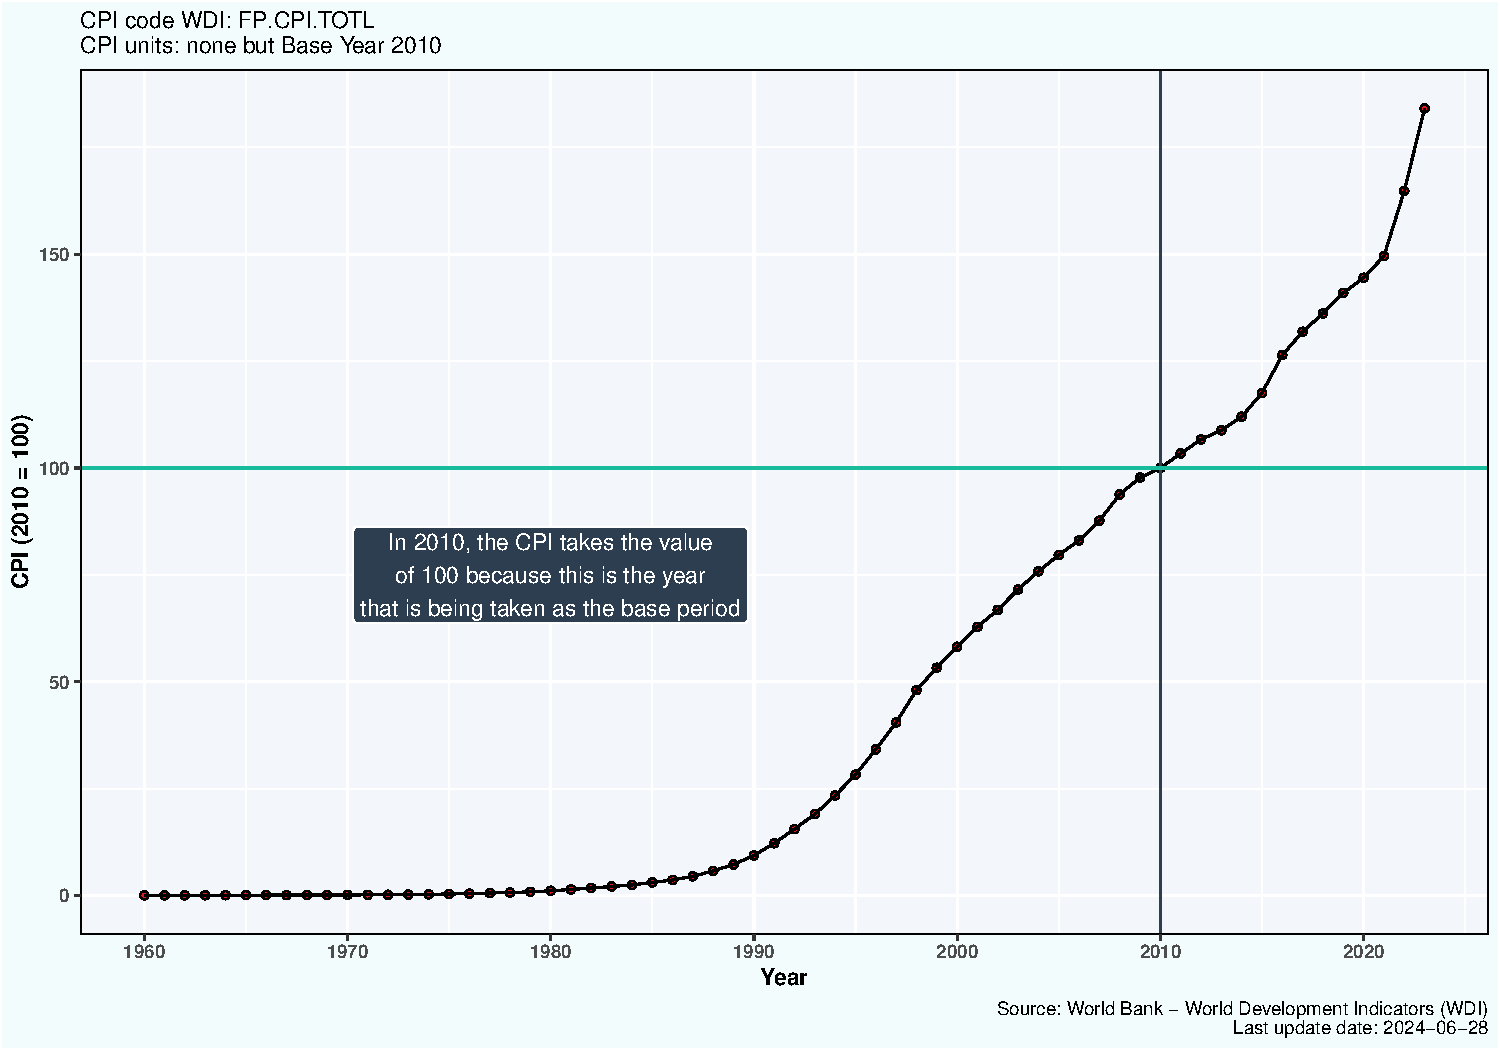
\includegraphics[width=0.85\textwidth,height=\textheight]{007_money_prices_exchange_rate_files/figure-beamer/fig-cpi-col-1.pdf}

}

\caption{\label{fig-cpi-col}Colombia Consumer price index (CPI)}

\end{figure}%
\end{frame}

\begin{frame}{}
\phantomsection\label{section-10}
\begin{figure}

\centering{

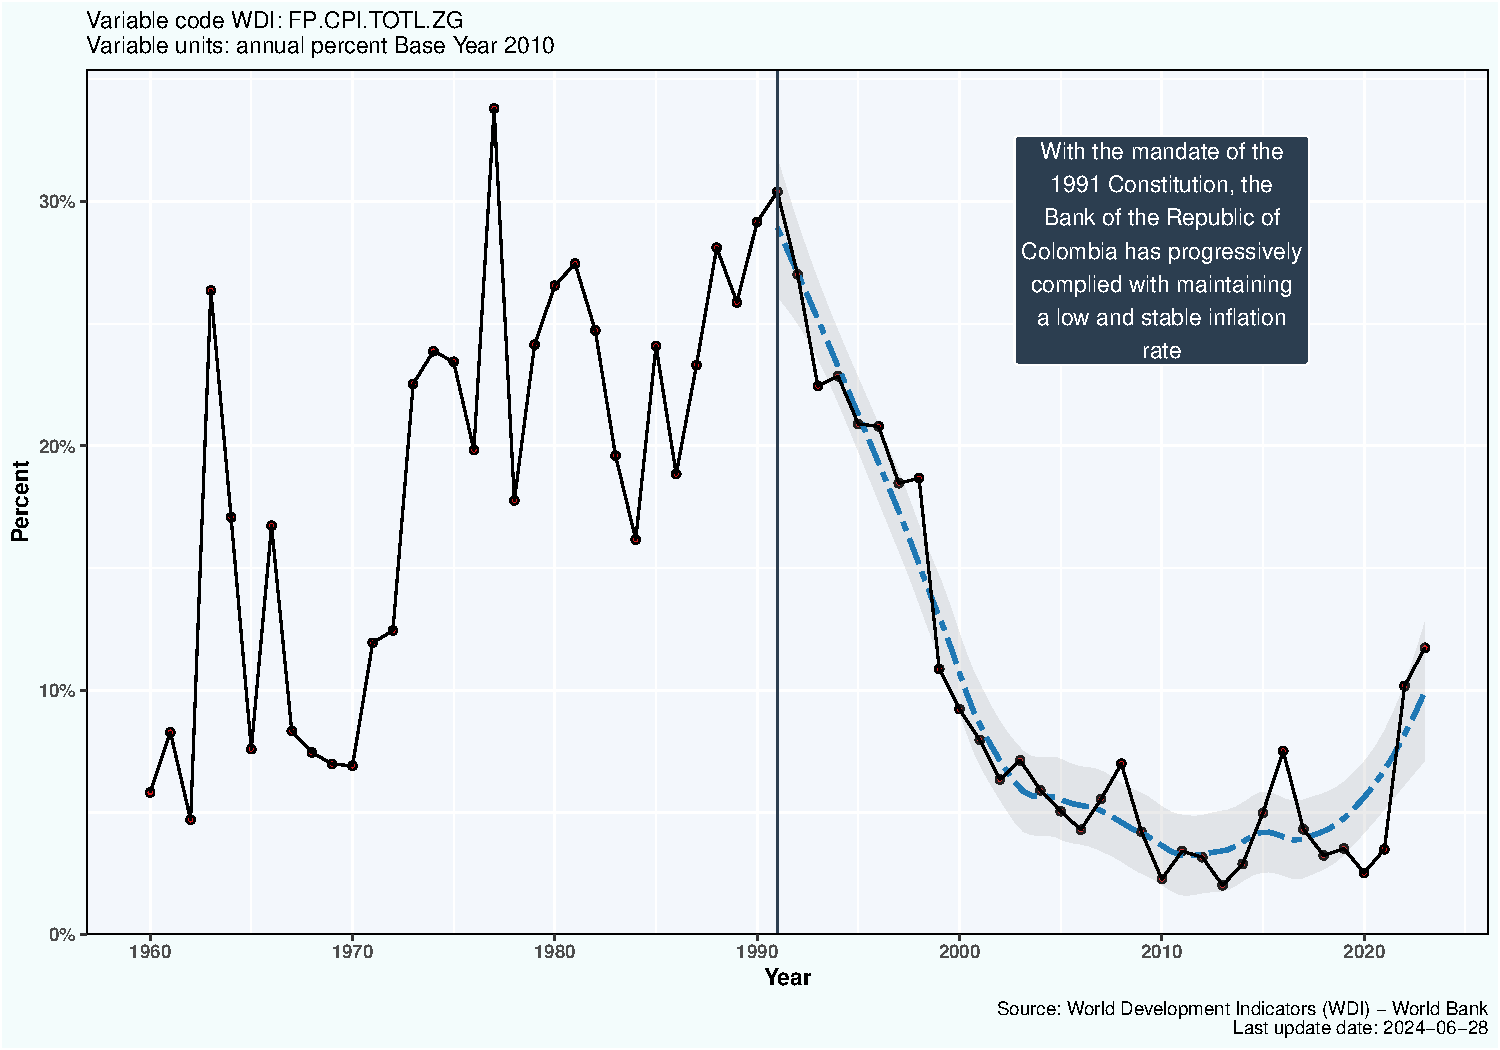
\includegraphics[width=0.85\textwidth,height=\textheight]{007_money_prices_exchange_rate_files/figure-beamer/fig-cpi-inflation-col-1.pdf}

}

\caption{\label{fig-cpi-inflation-col}Inflation using CPI for Colombia}

\end{figure}%
\end{frame}

\begin{frame}{}
\phantomsection\label{section-11}
\begin{itemize}
\item
  Calculating inflation using the \textbf{Consumer Price Index (CPI)}

  \begin{itemize}
  \item
    CPI annual periodicity

    \[Inflation_t = \frac{CPI_t - CPI_{t-1}}{CPI_{t-1}} \times 100\]
  \item
    CPI monthly periodicity

    \[Inflation_t = \frac{CPI_t - CPI_{t-12}}{CPI_{t-12}} \times 100\]
  \end{itemize}
\end{itemize}
\end{frame}

\section{Exchange Rate and TRM
COP/USD}\label{exchange-rate-and-trm-copusd}

\begin{frame}{}
\phantomsection\label{section-12}
\begin{itemize}
\item
  An exchange rate is the amount of \textbf{units of national currency}
  that must be given in exchange for a \textbf{unit of foreign currency}
\item
  If the exchange rate between COP\footnote<.->{Colombian peso according
    to ISO 4217 code} and USD\footnote<.->{United States dollar
    according to ISO 4217 code} is 3808 COP/USD, it means that 3808 COP
  must be given to obtain 1 USD
\item
  To have a reference of the exchange rate between COP and USD, the
  \textbf{``Superintendencia Financiera de Colombia (SFC)''} currently
  calculates and certifies an \emph{average} exchange rate called
  \textbf{``Tasa Representativa del Mercado (TRM)''} on a daily basis
\item
  Also it is important to take into account the following terminology:

  \begin{itemize}
  \tightlist
  \item
    \textbf{Devaluation}: TRM - COP/USD \((\Uparrow)\)
  \item
    \textbf{Revaluation}: TRM - COP/USD \((\Downarrow)\)
  \end{itemize}
\end{itemize}
\end{frame}

\begin{frame}{}
\phantomsection\label{section-13}
\begin{figure}

\centering{

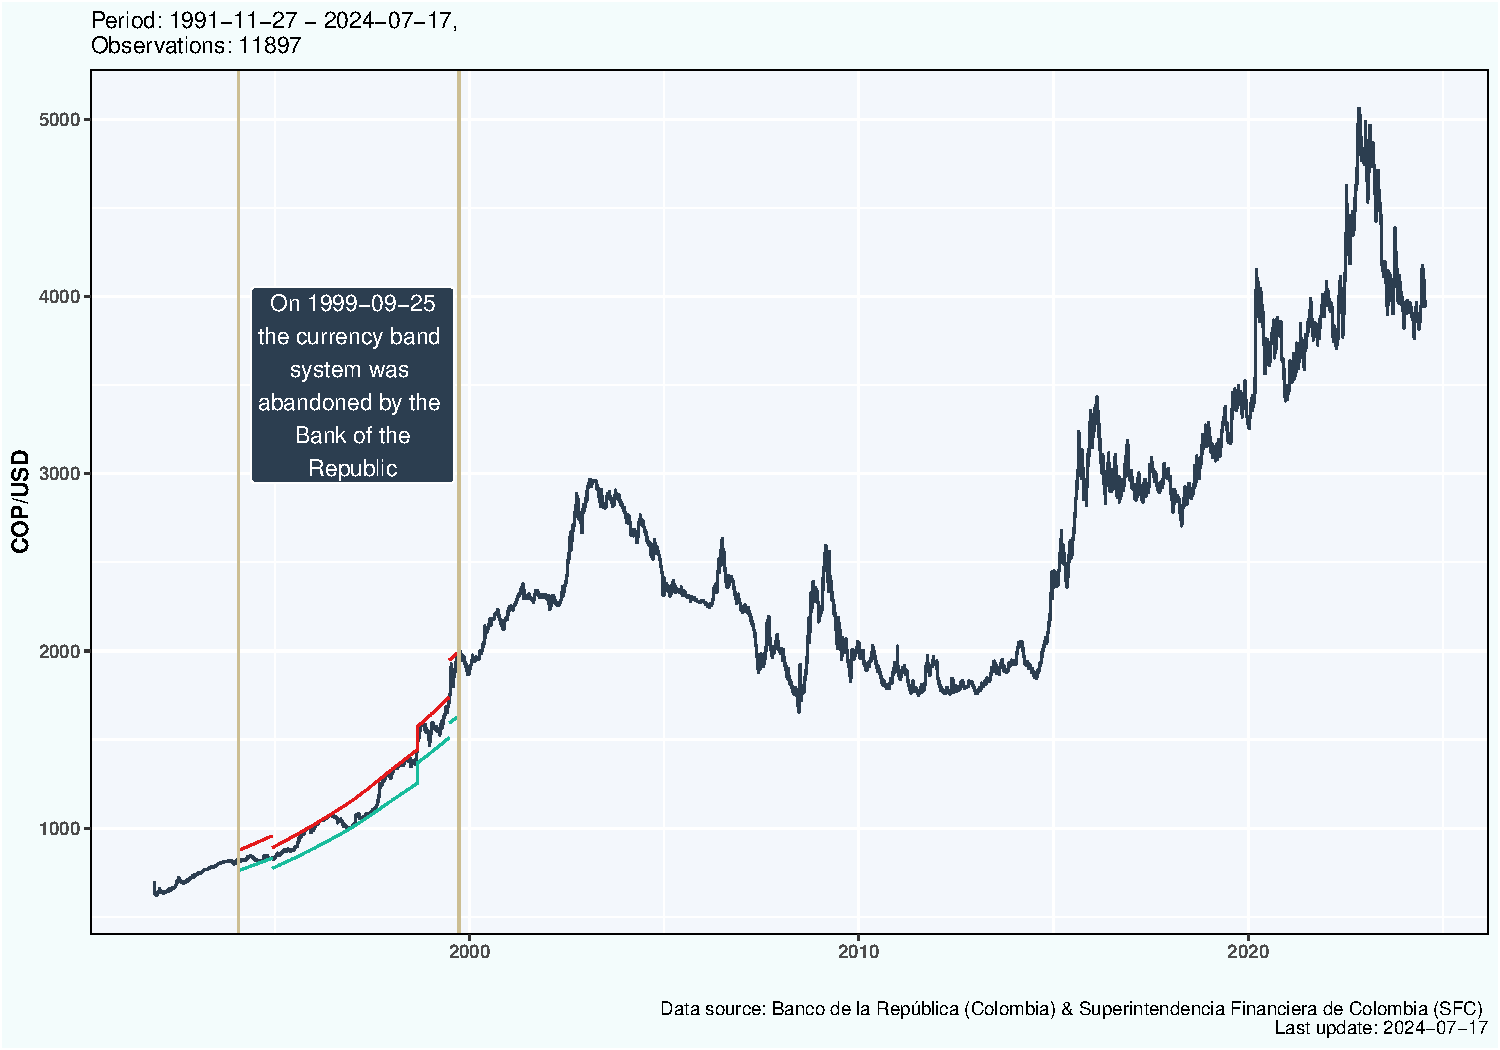
\includegraphics[width=0.85\textwidth,height=\textheight]{007_money_prices_exchange_rate_files/figure-beamer/fig-daily-trm-cop-usd-1.pdf}

}

\caption{\label{fig-daily-trm-cop-usd}Daily TRM (COP/USD)}

\end{figure}%
\end{frame}

\section{Monetary policy intervention
rate}\label{monetary-policy-intervention-rate}

\begin{frame}{}
\phantomsection\label{section-14}
\begin{itemize}
\item
  In the link
  \href{https://www.banrep.gov.co/es/estadisticas/tasas-interes-politica-monetaria}{\textbf{https://www.banrep.gov.co/es/estadisticas/tasas-interes-politica-monetaria}}
  on \textbf{2024-07-02} it was pointed out that:

  \begin{itemize}
  \item
    \emph{``La tasa de intervención de política monetaria o tasa de
    referencia es la tasa de interés mínima que el Banco de la República
    (BanRep) cobra a las entidades financieras por la liquidez que les
    suministra mediante las operaciones de mercado abierto (OMA). Esta
    tasa es el principal instrumento de intervención de política
    monetaria utilizado por el BanRep para afectar la cantidad de dinero
    que circula en la economía.''}
  \item
    Also the \emph{``tasa de intervención de política monetaria''} on
    \textbf{2024-07-02} was \textbf{11.25\%}
  \end{itemize}
\end{itemize}
\end{frame}

\begin{frame}{}
\phantomsection\label{section-15}
\begin{figure}

\centering{

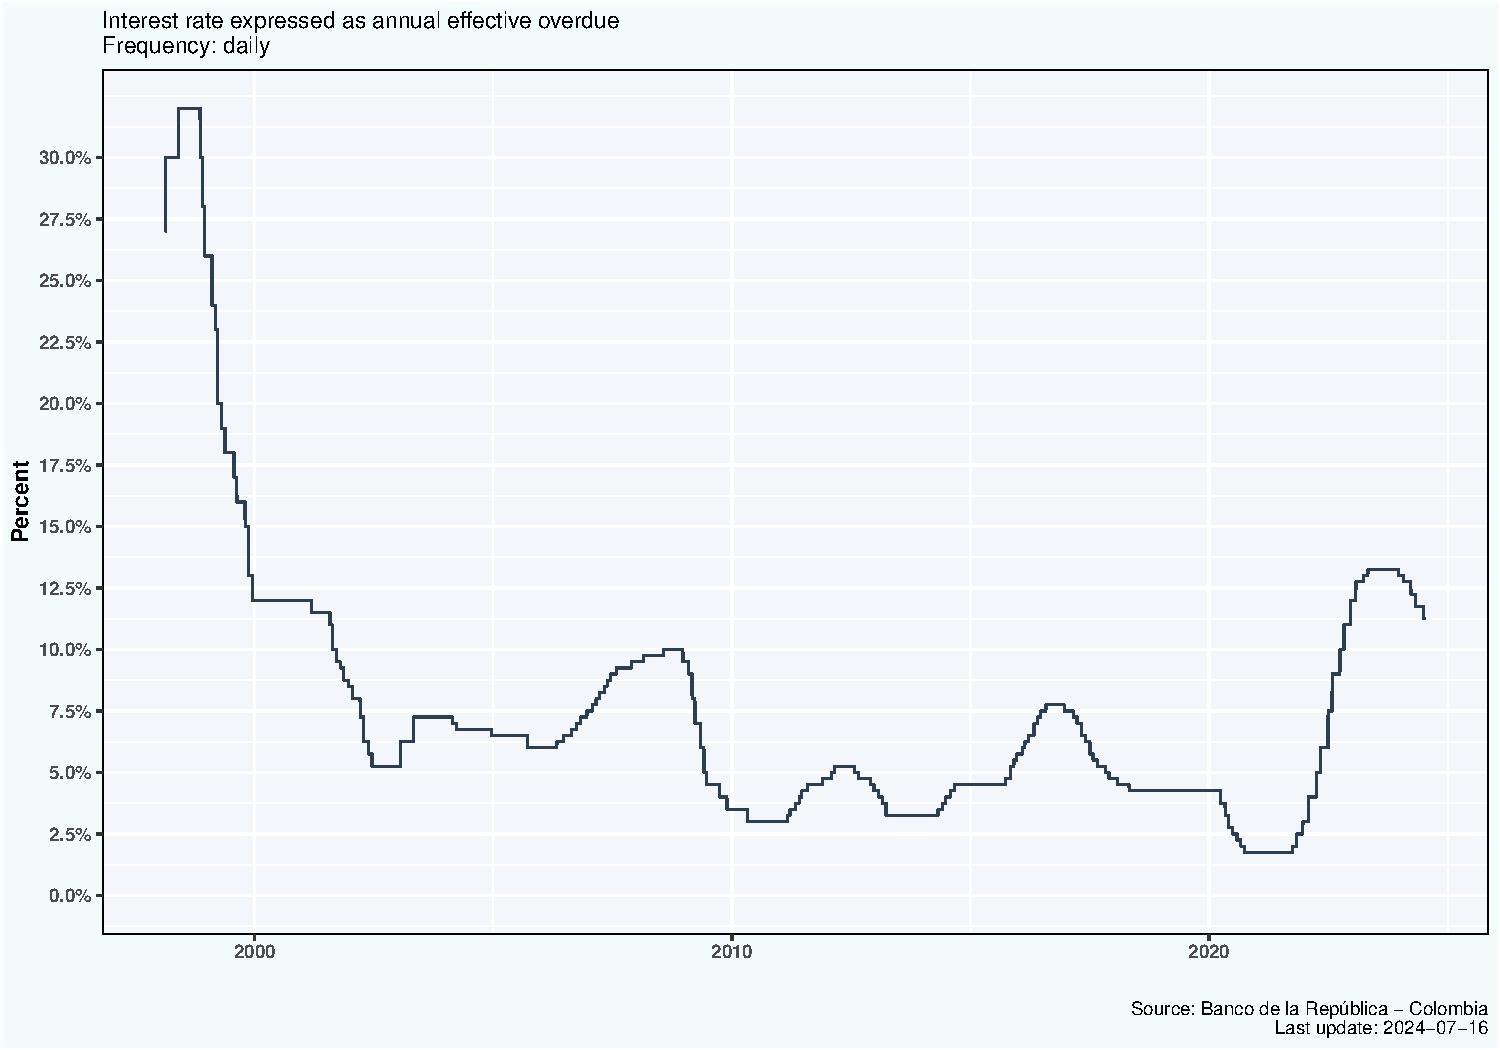
\includegraphics[width=0.85\textwidth,height=\textheight]{007_money_prices_exchange_rate_files/figure-beamer/fig-daily-pir-col-1.pdf}

}

\caption{\label{fig-daily-pir-col}Monetary policy intervention rate of
the Bank of the Republic (Colombia)}

\end{figure}%
\end{frame}

\begin{frame}{}
\phantomsection\label{section-16}
\begin{figure}

\centering{

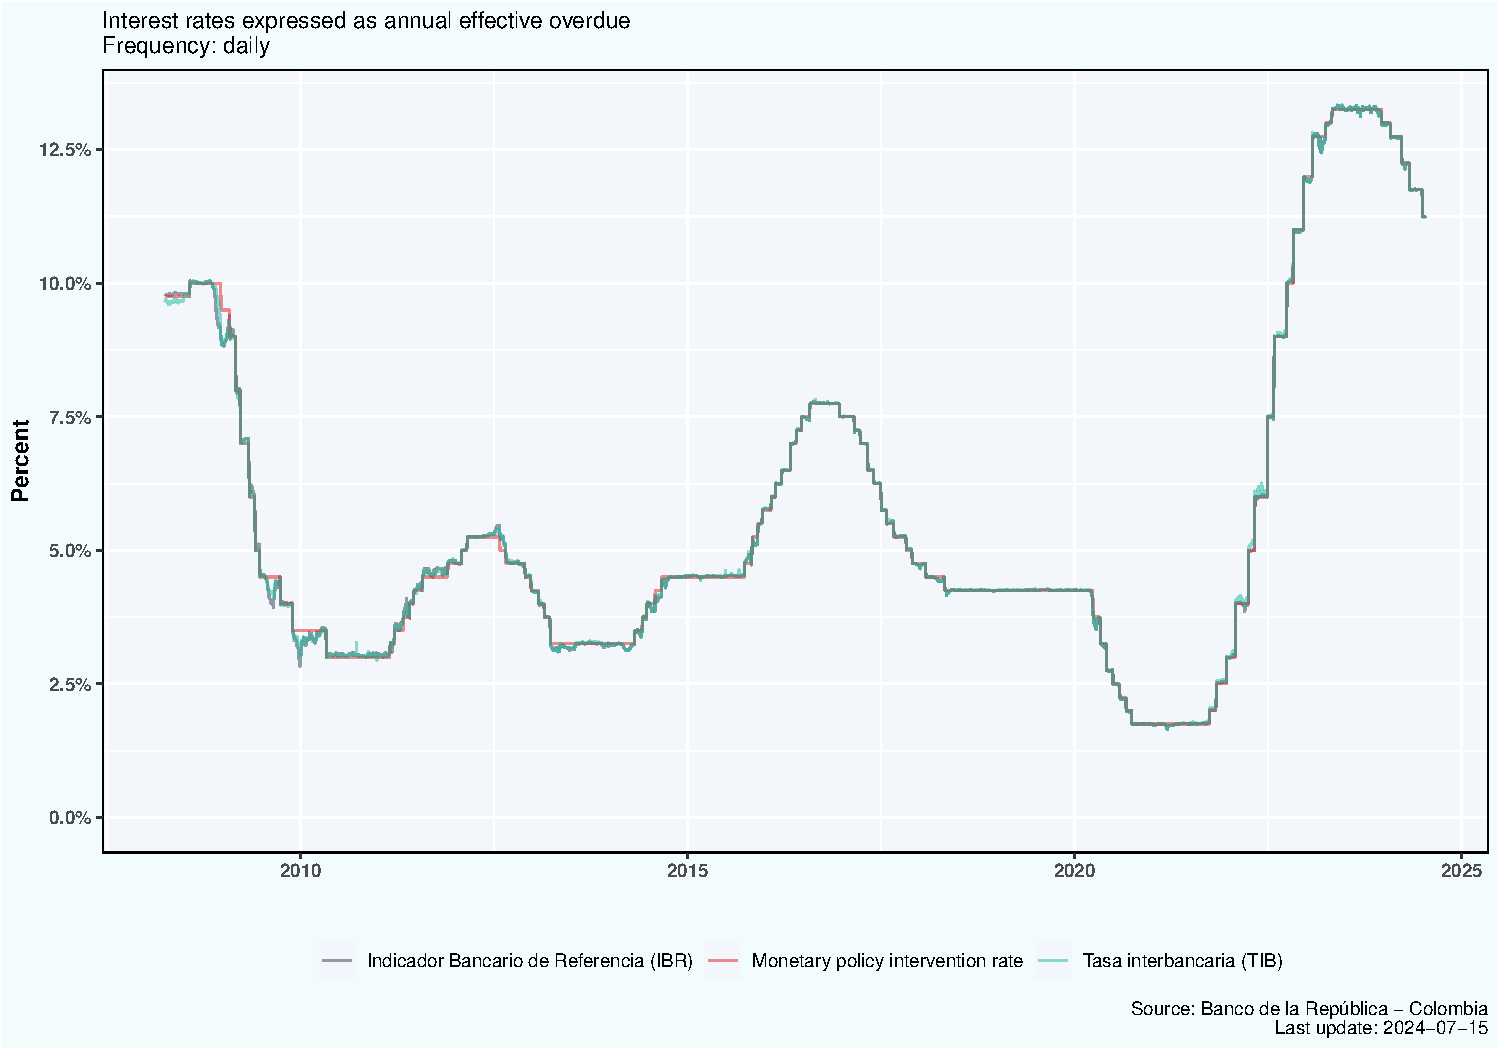
\includegraphics[width=0.85\textwidth,height=\textheight]{007_money_prices_exchange_rate_files/figure-beamer/fig-daily-pir-tib-ibr-col-1.pdf}

}

\caption{\label{fig-daily-pir-tib-ibr-col}Monetary policy intervention
rate, TIB and IBR}

\end{figure}%
\end{frame}

\begin{frame}{}
\phantomsection\label{section-17}
\begin{figure}

\centering{

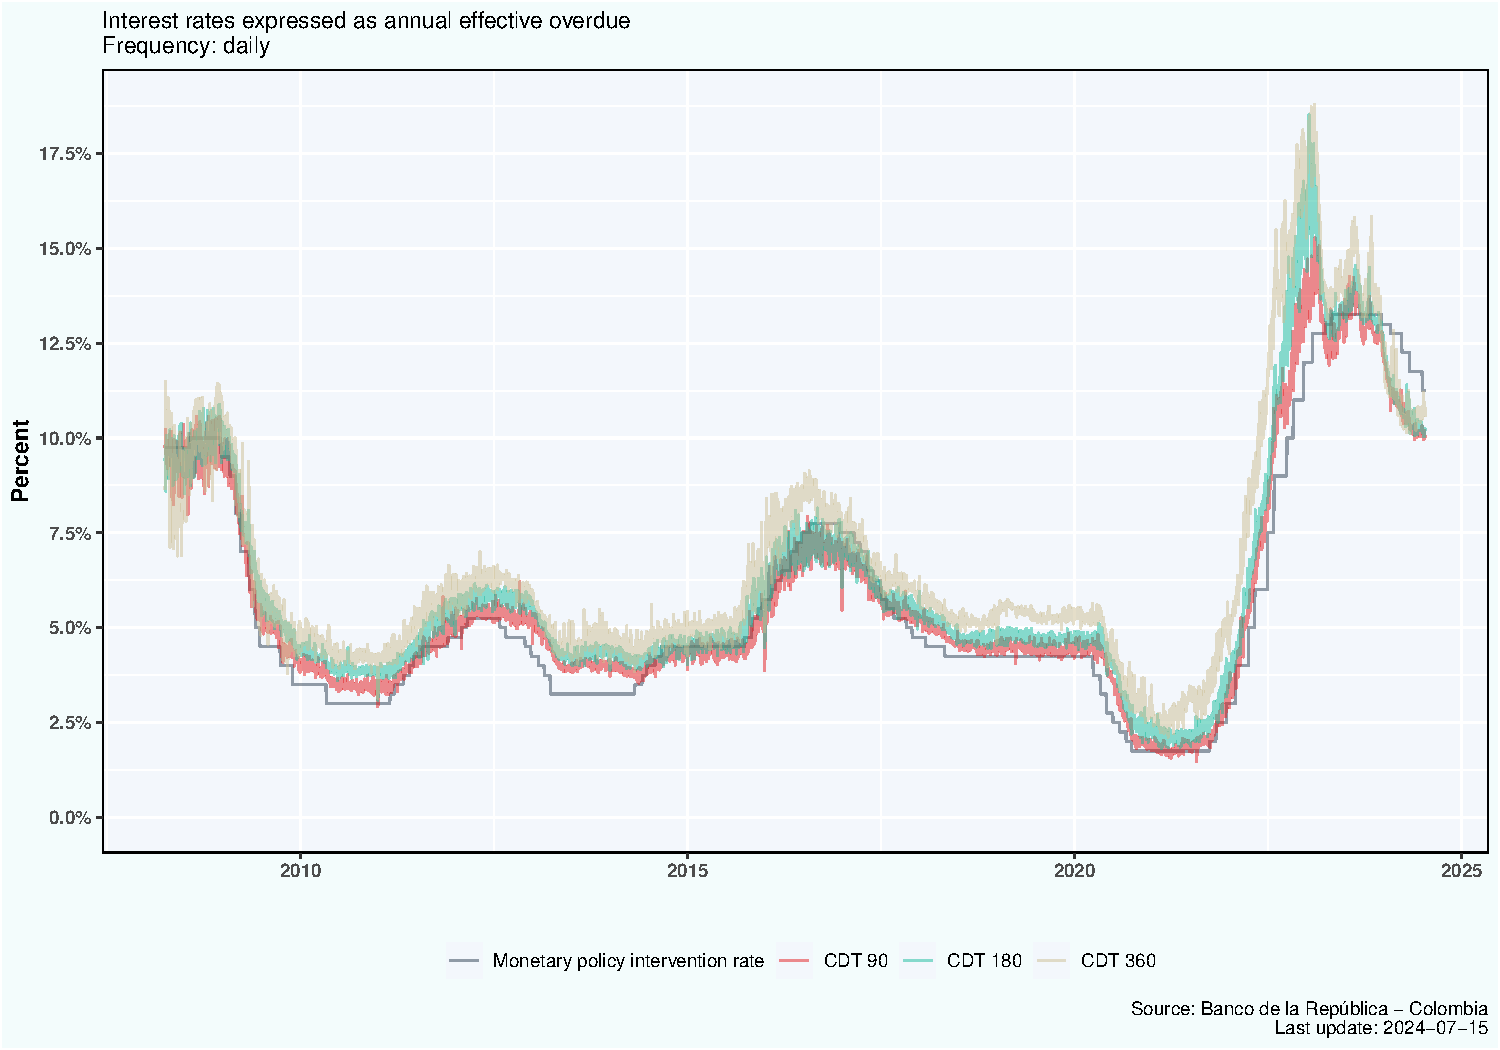
\includegraphics[width=0.85\textwidth,height=\textheight]{007_money_prices_exchange_rate_files/figure-beamer/fig-daily-pir-cdt-90-180-360-col-1.pdf}

}

\caption{\label{fig-daily-pir-cdt-90-180-360-col}Monetary policy
intervention rate and CDT interest rates}

\end{figure}%
\end{frame}

\section{Monetary policy transmission
channels}\label{monetary-policy-transmission-channels}

\begin{frame}{}
\phantomsection\label{section-18}
\begin{figure}

\centering{

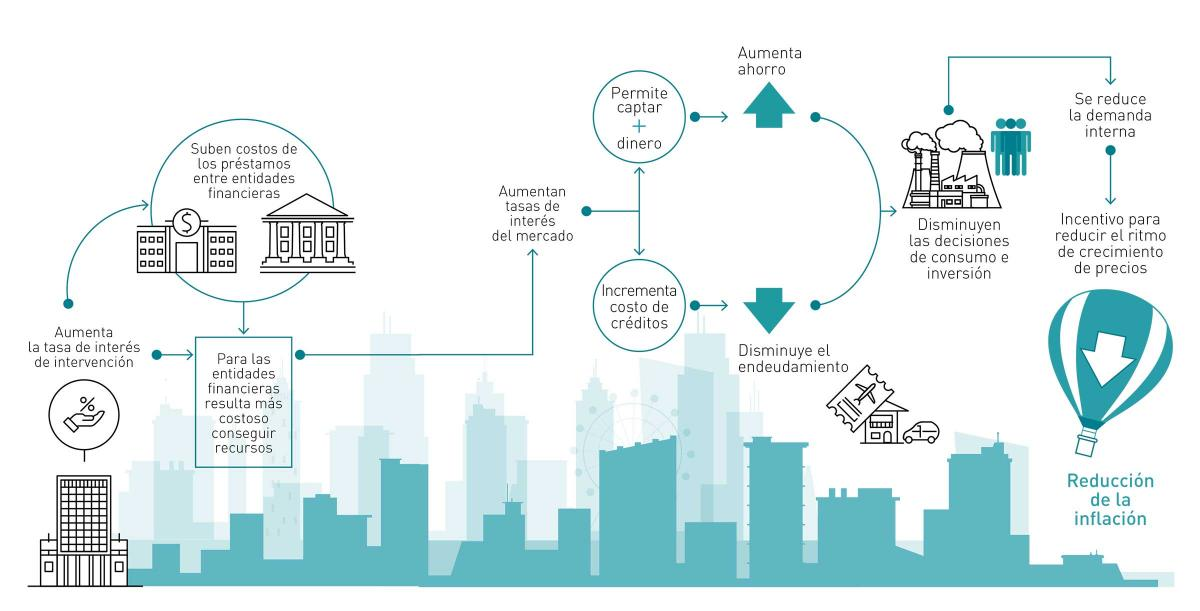
\includegraphics[width=4.6875in,height=4.6875in]{_000_images/007_econo_canales_transmision_1_tasa_interes_credito.jpg}

}

\caption{\label{fig-canal-tasa-interes-credito}\textbf{Interest rate and
credit} (\citeproc{ref-banrep_canales_2020}{Banrep 2020}, fig.~Canal De
Tasa De Interés Y De Crédito: Ejemplo Gráfico)}

\end{figure}%
\end{frame}

\begin{frame}{}
\phantomsection\label{section-19}
\begin{figure}

\centering{

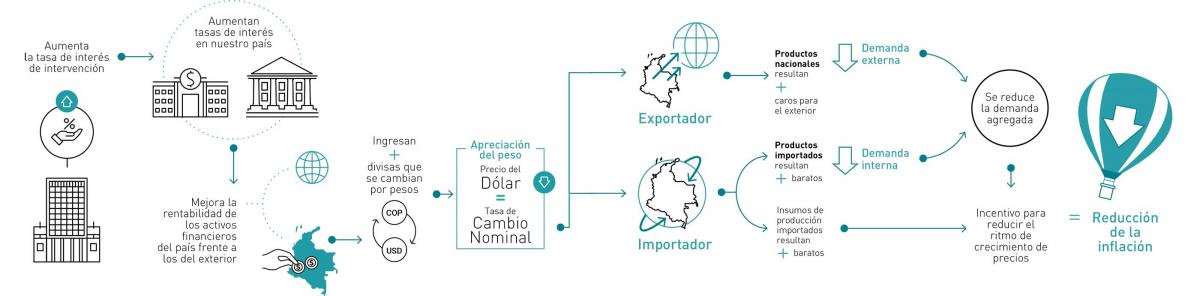
\includegraphics[width=4.6875in,height=6.25in]{_000_images/007_econo_canales_transmision_2_tasa_cambio.jpg}

}

\caption{\label{fig-canal-tasa-de-cambio}\textbf{Exchange rate}
(\citeproc{ref-banrep_canales_2020}{Banrep 2020}, fig.~Canal De Tasa De
Cambio: Ejemplo Gráfico)}

\end{figure}%
\end{frame}

\begin{frame}{}
\phantomsection\label{section-20}
\begin{figure}

\centering{

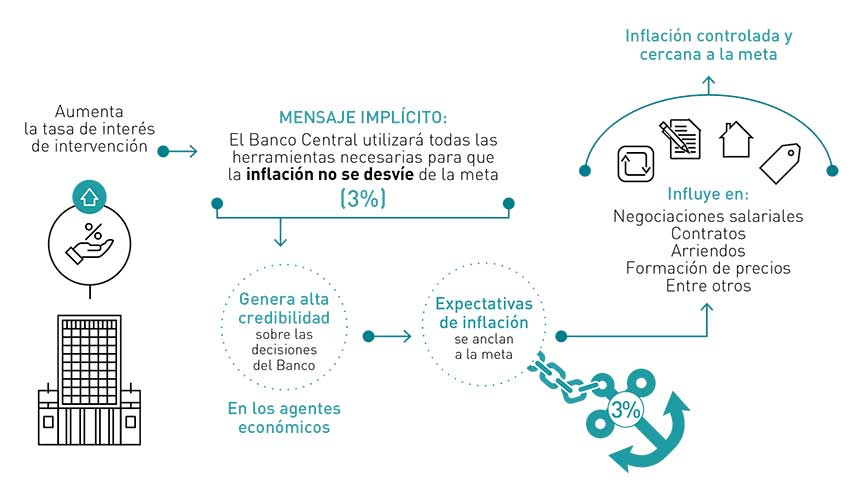
\includegraphics[width=4.16667in,height=4.16667in]{_000_images/007_econo_canales_transmision_3_expectativas.jpg}

}

\caption{\label{fig-canal-expectativas}\textbf{Expectations}
(\citeproc{ref-banrep_canales_2020}{Banrep 2020}, fig.~Canal De Las
Expectativas: Ejemplo Gráfico)}

\end{figure}%
\end{frame}

\section{Acknowledgments}\label{acknowledgments}

\begin{frame}{}
\phantomsection\label{section-21}
\begin{itemize}
\item
  To my family that supports me
\item
  To the taxpayers of Colombia and the
  \href{https://www.umng.edu.co/estudiante}{\textbf{UMNG students}} who
  pay my salary
\item
  To the \href{https://www.business-science.io/}{\textbf{Business
  Science}} and \href{https://www.rfordatasci.com/}{\textbf{R4DS Online
  Learning}} communities where I learn
  \href{https://www.r-project.org/about.html}{\textbf{R}} and
  \href{https://www.python.org/about/}{\textbf{\(\pi\)-thon}}
\item
  To the \href{https://www.r-project.org/contributors.html}{\textbf{R
  Core Team}}, the creators of
  \href{https://rstudio.com/products/rstudio/}{\textbf{RStudio IDE}},
  \href{https://quarto.org/}{\textbf{Quarto}} and the authors and
  maintainers of the packages
  \href{https://CRAN.R-project.org/package=tidyverse}{\textbf{tidyverse}},
  \href{https://CRAN.R-project.org/package=knitr}{\textbf{knitr}},
  \href{https://CRAN.R-project.org/package=kableExtra}{\textbf{kableExtra}},
  \href{https://CRAN.R-project.org/package=wbstats}{\textbf{wbstats}},
  \href{https://CRAN.R-project.org/package=tidyquant}{\textbf{tidyquant}},
  and
  \href{https://CRAN.R-project.org/package=tinytex}{\textbf{tinytex}}
  for allowing me to access these tools without paying for a license
\item
  To the \href{https://www.kernel.org/category/about.html}{\textbf{Linux
  kernel community}} for allowing me the possibility to use some
  \href{https://static.lwn.net/Distributions/}{\textbf{Linux
  distributions}} as my main
  \href{https://en.wikipedia.org/wiki/Operating_system}{\textbf{OS}}
  without paying for a license
\end{itemize}
\end{frame}

\section*{References}\label{references}
\addcontentsline{toc}{section}{References}

\begin{frame}[allowframebreaks]{References}
\phantomsection\label{refs}
\begin{CSLReferences}{1}{0}
\bibitem[\citeproctext]{ref-banrep_canales_2020}
Banrep. 2020. {``Canales de Transmisión de La Política Monetaria.''}
\emph{Banco de La República (Banco Central de Colombia)}.
\url{https://www.banrep.gov.co/es/canales-transmision-politica-monetaria}.

\bibitem[\citeproctext]{ref-cardenas_introduccion_2020}
Cardenas, Mauricio. 2020. \emph{Introducción a La {Economía}
{Colombiana}}. 4th ed. Alfaomega.

\bibitem[\citeproctext]{ref-dane_metodologigeneral_2019}
DANE. 2019. {``Metodología {General} Índice de {Precios} Al {Consumidor}
- {IPC}.''} Dirección de Metodología y Producción Estadística - DIMPE.
\url{https://www.dane.gov.co/index.php/estadisticas-por-tema/precios-y-costos/indice-de-precios-al-consumidor-ipc/ipc-informacion-tecnica}.

\bibitem[\citeproctext]{ref-herger_understanding_2019}
Herger, Nils. 2019. \emph{Understanding {Central} {Banks}}. Cham:
Springer International Publishing.
\url{https://doi.org/10.1007/978-3-030-05162-4}.

\bibitem[\citeproctext]{ref-ralph_practical_2015}
Ralph, Jeff, Rob O'Neill, and Joe Winton. 2015. \emph{A Practical
Introduction to Index Numbers}. Chichester, West Sussex: Wiley.

\bibitem[\citeproctext]{ref-banco_de_la_republica_central_2021}
República, Banco de la. 2021. {``A {Central} {Bank} {\textbar} {Banco}
de La {República}.''} \url{https://www.banrep.gov.co/en/node/7599}.

\end{CSLReferences}
\end{frame}




\end{document}
